\chapter{Specifikace}\label{ch:specification}

Z hlediska specifikace za základ je považovaná specifikace definovaná v bakalářské práci v kapitole \enquote{Specifikace informačního systému}~\cite{bachelorthesis}.
Zachovává se hlavní myšlenka – iterativní zpracovávání studentských projektů na základě komunikace dvou subjeků (vedoucího a studenta), jež postupně tvoří obsah projektu (viz obrázek~\ref{pic:main-communication-cycle}).

\begin{figure}[htbp]
   \centering
   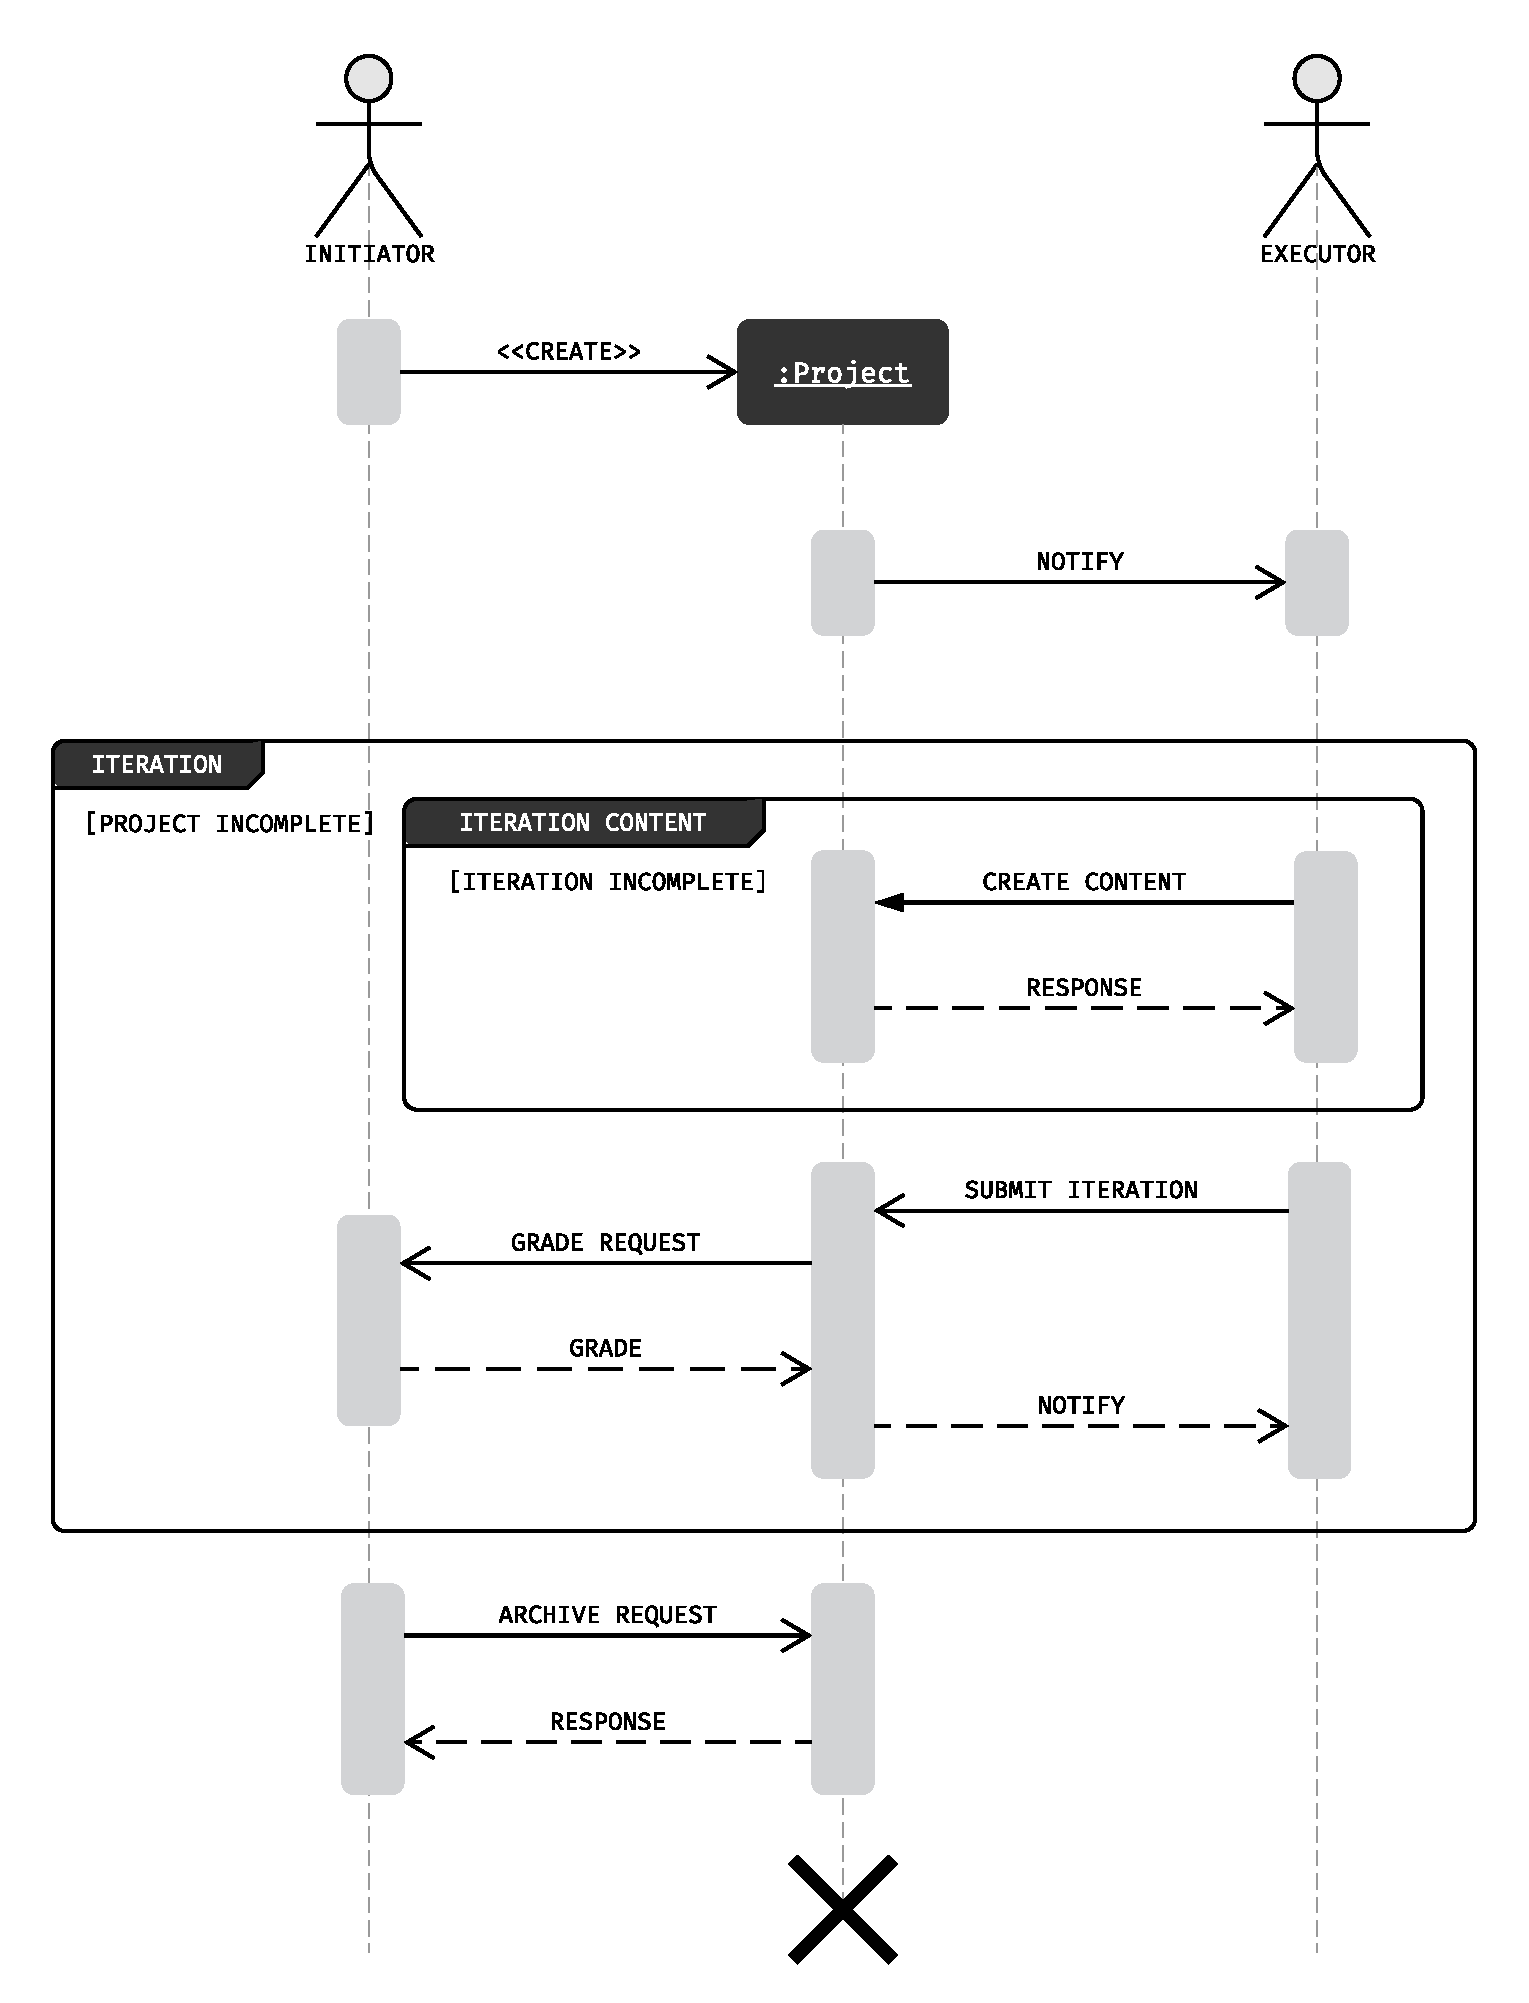
\includegraphics[max width=\textwidth]{assets/dia-seq-study-project-lifecycle}
   \caption[Zobecněný životní cycklus projektu]{Zobecněný životní cyklus projektu~\cite{bachelorthesis}}\label{pic:main-communication-cycle}
\end{figure}



\section{Požadavky na systém}

Požadavky na \g{IS} z přechozí práce jsou uměle upraveny dle aktuálních potřed, aby vynechaly méně prioriptní věci a byly vhodné pro vývoj na \g{MSA}.



\subsection{Funkční požadavky}

\begin{dl}
   \item[FP00] \textbf{Identita uživatelů} – uživatelé se mohou registrovat, přihlásit a vykonávat určité činnosti na základě přidělených práv.
   \item[FP01] \textbf{Globální role} – práva uživatelů jsou přidělována na základě rolí, administrátor systému má má neomezený přístup a má právo změnit roli uživatele.
   \item[FP02] \textbf{Uživatelská data} – aplikace umožňuje uživatelům prohlížet si svoje data a v případě nutnosti odstanit referenci na jejich osobu (odstranit účet).
   \item[FP03] \textbf{Upozornění} – aplikace posílá uživatelům relevantní upozornění na základě změn v \g{IS}.
   Uživatel takové upozornění může označit jako přečtenou/nepřečtenou, nebo odstranit.
   \item[FP04] \textbf{Projekt – životní cyklus} – aplikace umožňuje uživatelům zakládat projekty s definováním detailních interních informací.
   Projekt může být následně upravován až do jeho zániku (permanentní odstranění), nebo pozastavení (archivování na dobu neurčitou).
   Projekt lze z archvívu obnovit a pokračovat v úpravách.
   \item[FP05] \textbf{Projekt – správa dat} – aplikace umožňuje každému projektu definovat veřejná, skrytá (pouze pro účastníky projektu) a volitelně skrytá data.
   \begin{ul}
      \item {\textbf{Veřejná} – kategorie, název, věřejný popis, cleny týmu, tagy, status archivace.}
      \item {\textbf{Skrytá} – iterace a úkoly, interní popis, snímky iterací a ohodnocení.}
      \item {\textbf{Volitelně skrytá} – vakantní pozice, obsah.}
   \end{ul}
   \item[FP06] \textbf{Projekt – kategorie a tagy} – aplikace umožňuje každému projektu definovat kategorie a tagy, dle kterých se dá vyhledávat.
   Seznam kategorií je spravován administrátory \g{IS}.
   V případně prázdné ketegorie, se dá odstranit.
   \item[FP07] \textbf{Projekt – tým a role} – v rámci každého proejktu každý uživatel má určitou roli, která mu přiděluje oprávění pro prohlížení/úpravu projektu.
   \begin{ul}
      \item {\textbf{Vedoucí} – neomezený přístup k projektu, spravuje všechny detaily projektu (role, uživatele, popis, tagy apod.). Prvním vedoucím se stává uživatel, jenž projekt založil. Vedoucí může povolit/zakázat roli Náveštěvník a definovat nové role v týmu, které budou mít stejná práva, jako role Spolupracovník.}
      \item {\textbf{Spolupracovník} – podílí se na tvorbě obsahu projektu, nezasahuje do interní správy projektu (název, přístupová práíva apod.).}
      \item {\textbf{Návštěvník} – může prohlížet detaily projektu.}
   \end{ul}
   Z projektu lze odejít, pokud se nejedná o posledního uživatele s rolí Vedoucí.
   Vedoucí může povolit/zakázat nábor uživatelů na role, u kterých je uvedena kapacita.
   Pokud má uživatel status důveryhodného, může přidávat členy týmu bez jejich souhlasu.
   \item[FP08] \textbf{Projekt – vyhledávání} – aplikace umožňuje vyhledat projekt dle zadaných kriterií.
   \item[FP09] \textbf{Projekt – iterace a úkoly} –
   \item[FP10] \textbf{Projekt – Správa obsahu} – aplikace umožňuje vedoucím a spolupracovníkům tvořit obsah projektu.
   Obssah je členěn do částí – každá část má datovou složku a název interpretu, který bude datovou složku zpracovávat do vizuální podoby.
   Každá část může označovat jeden, či více úkolů za splněné.
   \item[FP11] \textbf{Projekt – snímky iterací} – stav obsahu projektu se da zafixovat a odeslat k ohodnocení u konkrétní iterace.
   \item[FP12] \textbf{Projekt – důvěryhodnost} – projekt je označen za důvěryhodný, pokud alespoň jeden z vedoucích je důvěryhodný.
\end{dl}



\subsection{Nefunkční požadavky}
\begin{dl}
   \item[FP00] \textbf{Veřejné \g{API}} – aplikace bude nabízet veřejné \g{API} s dokumentací pro vývoj aplikací.
   \item[FP01] \textbf{Dokumentace} – součástí \g{IS} je uživatelská a vývojářská dokumentace.
   \item[FP02] \textbf{Rozšiřitelnost} – aplikace je připůsobena dalšímu rozvoji a umožňuje škálovat jednotlivé části fukcionality dle zátěže.
   \item[FP03] \textbf{Uživatelské rozhraní} – uživatelské rozhraní je ve webové podobě a podporuje prohlížeč Google Chrome.
   Mobilní rozhraní není potřeba.
   \item[FP04] \textbf{Jazykové verze} – rozhraní je připraveno pro překlad do dalších jazyků.
   \item[FP05] \textbf{Úložiště dat projektů} – úložiště dat projektů bude možné konfigurovat před prvním spuštěním \g{IS}.
   Výměna úložiště se zachováním údajů během provozu \g{IS} není nutná.
\end{dl}





\TODO{Napsat testovací scénáře pro testování funkčnosti, viz kapitola Testování}
